\newpage
\section{Beratender Teil} \label{sec:beratender-teil}

\subsection{Essenzielle Eigenschaften bei Social Media Posts}
Social Media Posts bilden das Herzstück einer jeden Social Media Plattform.
Dabei können sich, je nach Plattform, die Social Media Beiträge merkbar unterschieden.
So setzt Instagram, als ausgewählte Social Media Plattform, ausschließlich den Schwerpunkt auf visuelle Beiträge, welche i. d. R. aus einem Foto oder (Kurz-) Video und einem Text unter dem visuellen Element bestehen.
Damit ein Beitrag auf einer Social Media Plattform gut ankommt und Klicks generiert, gibt es einige Kriterien die zu beachten sind, bzw. Eigenschaften die zu erfüllen sind.

Das erste Kriterium beschreibt die Kreativität und die Einzigartigkeit von Beiträgen.\footcite{kaplan_users_2010,keller_building_1993}
Dabei geht es inhaltlich darum, dass besonders auffällige Beiträge, im Sinne der Authentizität, Ausgefallenheit, oder Individualität eher bei Benutzern der Plattform auf Interesse stoßen als Beiträge, die sich nicht von der Masse abheben.
Ein Beispiel hierfür ist die Abbildung des traditionellen Zubereitungsprozesses einer Pizza, die mit einer besonderen Tomatensauce sowohl visuell als auch schriftlich beworben wird.\footcite{green_role_2000}

Ein weiteres Kriterium ist die Definition einer Zielgruppe.\footcite{kotler_marketing_management}
Dies ist erheblich wichtig, da mit der Auswahl einer Zielgruppe entsprechende gewählte Artikulation notwendig ist.
Ebenso wirkt sich das auf den Stil der Beiträge aus.
Ein italienisches Restaurant, das sich durch verschiedene Faktoren wie eine lockere Atmosphäre, günstige Preise und spezielle Angebote an eine junge Zielgruppe wendet, legt dabei visuell als auch sprachlich andere Schwerpunkte bei den Beiträgen als ein vergleichbares Restaurant, das auf eine Zielgruppe mit gesteigerter Kaufkraft ausgerichtet ist.

Social Media Beiträge, aus Sicht eines Gastronomen, sollten immer eine Konversionsorientierung haben.\footcite{website_quality_customer_satisfaction}
Genauer gesagt, definiert die Konversionsorientierung ein Call-to-Action, bei dem der Kunde kommunikativ aufgefordert wird auf einen Link zu klicken, ein Tisch zu reservieren oder vergleichbare interaktionen zu tätigen.
Eine Strategie, die das Call-to-Action Prinzip verstärkt ist die Verlustaversion, im Sinne von Marketingkampagnen, die auf ein zeitlich, oder physisch begrenztes Angebot hinweisen.\footcite{jstor_example}
Ein Beispiel für diese Eigenschaft wäre das Bewerben eines zeitlich begrenzten Angebotes von drei Pizzen im Preis von zwei Pizzen.

Ansprechende Bildbeiträge spiegeln ein weiteres, wichtiges Kriterium wider, um die Aufmerksamkeit von Nutzern zu erlangen.\footcite{davidson_social_media}
So geht aus einer Studie von Sabate et al. aus dem Jahr 2014 hervor, dass visuelle Inhalte weitaus mehr Engagement erzeugen, als rein auf Text basierte.
Dabei sollten die Bilder auch aussagekräftig sein und mit der Eigenschaft der Kreativität und Einzigartigkeit synergieren.\footcite{sabate_factors}

Die persönliche und emotionale Ansprache der Zielgruppe und das Erzählen einer Geschichte sind bei dem Social Media Marketing ebenfalls wichtige Eigenschaften, die in Beiträgen beachtet werden sollten.
Gemeint sind dabei Inhalte, die Emotionen, wie z. B. Vorfreude, oder Hunger, bei den Social Media Nutzern auslösen.
Erzählungen über das Team, die Philosophie, die Geschichte des Restaurants, oder die Besonderheit der Zutaten sind hier wichtige Aspekte in der Kommunikation mit den Kunden auf den Social Media Plattformen, um diese als Kunden zu gewinnen.\footcite{book}

Zwei weitere Aspekte, die ebenfalls großen Einfluss auf das Social Media Marketing nehmen, sind zu einem der Ereignisbezug und zum anderen der Trendbezug.
Dabei beziehen sich diese beiden Punkte auf Aspekte, die einen Bezug zur aktuellen Saison, wie beispielsweise in Form der Jahreszeiten, oder zu gegenwärtigen Ereignissen, wie etwa einer Fußball-Weltmeisterschaft, herstellen.
Der Bezug auf solche Aspekte führt generell zu einem höheren Engagement.
Ein Beispiel für einen saisonalen Bezug wäre die Bewerbung einer besonderen Pizza, die nur während der Wintersaison erhältlich ist.
Ein weiteres Beispiel für den Trendbezug wäre die Reaktion auf die Ergebnisse der deutschen Nationalmannschaft, bei der aus Fußballspielsiegen Rabatte für Pizzabestellungen resultieren.\footcite{inbook}

Eine weitere, essenzielle Eigenschaft spiegelt die auf Social Media ausgerichtete Optimierung der Inhalte wider.
Diese Eigenschaft behandelt Hashtag-Strategien, welche relevant sind für die Auffindbarkeit der Social Media Beiträge, und wie die Strukturierung der Inhalte zu erfolgen hat, um vom Social Media Algorithmus bevorzugt angezeigt zu werden.\footcite{social_media_marketing}

Darüber hinaus sollte bei jedem Social Media Beitrag die Mehrsprachigkeit und Lokalität betrachtet werden.
Beide Aspekte zielen auf ein höheres Engagement.
Durch den möglichen Einsatz von Mehrsprachigkeit, wie z. B. neben der deutschen Sprache auch noch die englische Sprache, und den Bezug auf die Lokalität, wie z. B. auf lokale Sport Events oder kulturelle Besonderheiten, kann eine höhere Zielgruppe angesprochen werden, was wiederum zu einer höheren Nachfrage führen würde.\footcite{global_marketing_advertising}

Zusammengefasst wurden folgende Eigenschaften betrachtet und als relevant für Social Media Posts designiert: „Kreativität“, Einzigartigkeit, „Zielgruppenorientierung“, Konversionsorientierung“, „Bildbeiträge“, „persönliche und emotionale Ansprache“, „Story telling“, „Ereignis- und Trendbezug“, „Social-Media-Optimierung“, „Strukturierung der Posts“, „Mehrsprachigkeit“ und „Lokalität“.
Diese Eigenschaften werden als fundierte Basis für die Entwicklung und Optimierung der Prompt des LLMs bezogen.

\subsection{Entwicklung eines Erstenwurfs für das Applikationsdesign}\label{subsec:entwicklung-eines-erstenwurfs-fuer-das-applikationsdesign}
In diesem Kapitel wird der Erstentwurf für das Applikationsdesign vorgestellt.
Der Erstentwurf beschreibt sowohl die Frontend- als auch die Backend-Architektur der Applikation.

\textbf{Frontend}\newline
Das Frontend stellt den Interaktionsbereich für den Benutzer dar.
Entsprechend ist es wichtig, dass das Frontend übersichtlich und intuitiv gestaltet ist.
Dabei ist es entscheidend, die komplexen Zusammenhänge der Applikation und abgebildeten Prozesse so zu visualisieren, dass der Benutzer nicht überfordert wird.
Die gesamte \ac{UX} soll so gestaltet sein, dass der Benutzer durch die Applikation geführt und dadurch die Akzeptanz der Applikation erhöht wird.

Zusätzlich soll sich die Applikation an die Corporate Identity des Unternehmens anpassen.
Dies soll durch die Verwendung der Unternehmensfarben in der Applikation und des Logos erreicht werden.

Zur Umsetzung gilt folgendes zu beachten:
\begin{itemize}
    \item Das DISH POS typische Orange soll als primäre Farbe verwendet werden.
    \item Als sekundäre Farben sollen Grau- und Blautöne verwendet werden.
    \item Die Farben sollen so gewählt werden, dass sie die Aufmerksamkeit des Benutzers auf wichtige Elemente lenken.
    \item Unternehmens- und Applikationslogos müssen an strategischen Stellen platziert werden.
\end{itemize}
\newpage

Aus den genannten Anforderungen wurden folgende Design-Elemente abgeleitet:

\textbf{Landing Page Darstellung und wiederkehrende Elemente}\newline
Das Konzept zur Landing Page besteht aus mehreren runden Interaktionselementen (Bubbles), welche die verschiedenen Funktionen der Applikation repräsentieren.
Dabei werden die wichtigen Funktionen, wie z. B. die Generierung von Social Media Content, durch eine größere Bubble hervorgehoben.
Durch den Größenunterschied der Bubbles kann die Prominenz der Funktionen visualisiert werden.
Als zentrales, wiederkehrendes Element über alle Seiten hinweg, wird eine Textausgabe zentral platziert, welche den Benutzer durch die Applikation führt.
Diese Textausgabe fungiert dabei als interaktive Komponente, die dem Benutzer ein personalisiertes Erlebnis bietet.
Der Navigationsbereich wird als Sidebar auf der linken Seite platziert, erreichbar über ein Burger-Icon.
Wie im \ac{UX} Design vorgesehen, wird das DISH POS Logo daneben platziert, wodurch es ein strategisch platziertes Element darstellt.
Zuletzt findet sich ein Login Icon in der oberen rechten Ecke, welches den Benutzer zum Login-Bereich führt.
Insgesamt ist die Darstellung minimalistisch gehalten, um den Benutzer auf die wichtigsten Elemente zu fokussieren.\footnote{Siehe Anhang, Abbildung \ref{fig:landing-page-concept}.}

Das aus dem Entwurf abgeleitete Design zeigt zusätzlich, dass durch entsprechende Farbgebung die Corporate Identity des Unternehmens eingebunden wird.\footnote{Siehe Anhang, Abbildung \ref{fig:landing-page}.}

\textbf{Dialog Darstellung}\newline
Die Dialog-Darstellung strukturiert sich durch ein zentrales Eingabefeld, in welchem der Benutzer durch einen geführten Dialog mehrere Fragen beantwortet.
Die dadurch gesammelten Eingaben werden später in der Generierung von Social Media Content verwendet, indem diese systematisch in die Prompts einfließen.
Das zentrale Textausgabeelement wird durch eine Fortschrittsanzeige ergänzt, welche den Benutzer über den aktuellen Stand des Dialogs informiert.
Dadurch wird erreicht, dass der Benutzer jederzeit über den Fortschritt informiert ist und dadurch die Akzeptanz der Applikation erhöht wird.
Nach dem Beantworten einer Frage wird der Benutzer durch eine Animation auf die nächste Frage hingewiesen.
Dadurch wird die minimalistische Darstellung der Anwendung beibehalten und eine übermäßige Informationsflut vermieden.\footnote{Siehe Anhang, Abbildung \ref{fig:dialog-concept}.}

Im detaillierten Design wird durch den Einsatz der DISH POS Farben die Benutzbarkeit weiter verstärkt.
Durch das Färben der weiterführenden Buttons in Orange bzw. das blaue Hervorheben für ein Navigieren in vorherige Schritte, wird eine wiederkehrende Designkomponente eingeführt.
Zudem wird durch das umgangssprachliche Formulieren, sowohl der Fragen als auch der Navigation, eine persönliche Ansprache an den Benutzer gewährleistet.
Ebenso findet sich die primäre orangene Farbe in der Fortschrittsleiste wieder, wodurch die Corporate Identity des Unternehmens eine strategische Position erfährt. \footnote{Siehe Anhang, Abbildung \ref{fig:dialog-page}.}

\textbf{Post Editor Darstellung}\newline
Der Post Editor stellt die komplexeste Komponente der Applikation dar.
Dieser gliedert sich in zwei Hauptbereiche, dem eigentlichen Editor und einer Vorschau der generierten Inhalte.
Der Editor ist dabei auf die minimalen Funktionen reduziert, um den Benutzer nicht zu überfordern.
Jede Eingabe ist dabei als eigenes Element dargestellt und beinhaltet die zuvor generierten Texte und Bilder.
Über den Editor kann der Nutzer die generierten Inhalte und Einstellungen anpassen, darunter den Zeitplan, den Text und das Bild.
Die Vorschau zeigt den geplanten Post im Design der Zielplattform, beispielsweise dargestellt für Instagram.\footnote{Siehe Anhang, Abbildung \ref{fig:editor-concept}.}

Im detaillierten Design wurden die DISH POS Farben in den Editor integriert, konsistent zu den bisherigen Darstellungen.
Abweichend vom initialen Konzept wurde zusätzlich ein Bereich für die Eingabe der Call-to-Action hinzugefügt.\footnote{Siehe Anhang, Abbildung \ref{fig:editor-page}.}

\textbf{Kalender Darstellung}\newline
Der Kalender erlaubt dem Nutzer die geplanten Posts zu verwalten und zu bearbeiten.
Dieser strukturiert sich Grundlegend durch eine Übersicht der aktuellen Woche, welche über eine Navigation durch die Wochen erweitert werden kann.
Jede Woche beinhaltet eine Kachel je Post, welche Information darüber enthält, wann der Post veröffentlicht wird und welcher Inhalt geplant ist.
Zudem ist für den User ersichtlich, auf welcher Plattform der Post veröffentlicht wurde.
Über Chips in der Fusszeile ist für den Nutzer transparent, ob ein Post veröffentlicht wurde, ob dieser geplant ist oder ob ein Entwurf vorliegt.
Dabei wird jeder Status in einer eigenen Farbe dargestellt, um einen schnellen Überblick zu gewährleisten.
Das zentrale Textausgabeelement wird in den oberen rechten Bereich verschoben, um den Fokus auf die Kalenderansicht zu legen, dabei jedoch weiterhin präsent zu sein.
Darüber werden dem Nutzer, in Anlehnung an die Landing Page, Bubbles mit den wichtigsten Funktionen der Kalenderansicht angezeigt.\footnote{Siehe Anhang, Abbildung \ref{fig:calendar-concept}.}

Abweichend zum Konzept wurde die Darstellung in der detaillierten Ansicht auf ein Icon für die Plattform reduziert.
Zudem wurde die Navigation durch den Kalender visuell reduziert, da davon auszugehen ist, dass nutzer selten weitreichende Zeiträume im Kalender betrachten werden.
Diese ist in der Standardansicht versteckt und wird über ein Hover-Element sichtbar.\footnote{Siehe Anhang, Abbildung \ref{fig:editor-page}.}

Als technische Basis für das Frontend wird, als Ergebnis der vorangegangenen Recherche, Vue.js verwendet.
Dieses wird zum Betrieb im Kubernetes Engine Cluster bereitgestellt.
Für den Betrieb im Kubernetes Cluster muss die Software Architektur Stateless sein, um mit der Skalierung kompatibel zu sein.
Eine Stateless-Architektur bedeutet, dass die Applikation keine Zustände speichert.
Würde die Applikation Zustände speichern, müssten diese bei einer Skalierung auf mehrere Instanzen synchronisiert werden, was zu einem erhöhten Aufwand führen würde.

Um die Applikation im Kubernetes Cluster hosten zu können, erfolgt das Verpacken der Vue.js Applikation in ein Docker-Image über den Google Cloud Build Service.\footcite{google_cloud_build}

Das daraus erzeugte Docker-Image wird in den Google Kubernetes Engine Cluster genutzt und entsprechend gestartet.
Dabei wird eine Deployment-Struktur, bestehend aus einem Load Balancer Service, sowie mindestens zwei Pods erstellt.
Der Load Balancer wird für externe Zugriffe konfiguriert und leitet die Anfragen an die Pods weiter.
Der Betrieb, mit mindestens zwei Pods, gewährleistet eine hohe Verfügbarkeit der Applikation und ermöglicht eine einfache Skalierung.
In der Entwicklungsphase ermöglicht der Multi-Pod-Betrieb ein frühes Testen von Load-Balancing und Skalierung, sowie die Überprüfung der Stateless-Architektur.

Zusätzlich enthält das Deployment sowohl Konfigurations- als auch Secrets-Dateien, um die Applikation zu konfigurieren und sensible Daten zu schützen.

\textbf{Backend}\newline
Ziel der Backend-Architektur ist es, die Datenhaltung und -verarbeitung zu gewährleisten und die benötigten Aufrufe zu anderen Komponenten zu ermöglichen.
Im Rahmen dieses Erstenwurfs wird zunächst ein einzelner Service konzipiert, der die Datenhaltung und -verarbeitung übernimmt, genannt \ac{SMC} Service

Der \ac{SMC} Service stellt eine \ac{REST} \ac{API} bereit, welche die Kommunikation mit dem Frontend ermöglicht.
Die \ac{REST} \ac{API} setzt sich aus verschiedenen Endpunkten zusammen, welche jeweils die verfügbaren Ressourcen und Aktionen beschreiben.

Folgende Ressourcen stellt der Service bereit:
\begin{itemize}
    \item \textbf{/generate-content} - POST: Dieser Endpunkt dient der generierung und Speicherung von Social Media Content.
    \item \textbf{/get-content} - GET: Dieser Endpunkt ermöglicht das Abrufen von generiertem Social Media Content.
\end{itemize}

Die implementierung des \ac{SMC} Services erfolgt über das Python Framework Django\footcite{djangoproject}.
Zur Kommunikation mit den Google Cloud Services wird die Google Cloud Python SDK\footcite{googlecloudpython} verwendet.

Mithilfe der Google Cloud Python \ac{SDK} und entsprechender Konfiguration des API Clients wird die Kommunikation mit den als Cloud Service gehosteten Text-to-Text- und Text-to-Image-Modellen ermöglicht.
Der POST Endpunkt wird vom Frontend aufgerufen, sobald der Benutzter seine Eingaben im Frontend abgeschlossen hat und den Social Media Content generieren möchte.
Anschließend werden die Eingabeparameter über ein \ac{HTTP} Request-Body Objekt im \ac{JSON} Format an den \ac{SMC} Service gesendet.
Dieser verarbeitet den Request und routet diesen an den zuständigen POST Endpunkt.
Über den POST Endpunkt wird anschließend durch Verwendung der Google Cloud \ac{REST} \ac{API} ein weiterer \ac{HTTP}-Request and den Text-to-Text-Modell Cloud Service gesendet.
Der Text-to-Text-Modell Cloud Service generiert anschließend aus den Eingaben einen finalen Eingabeprompt und sendet eine \ac{HTTP}-Response mit den Ergebnissen der Generierung als HTTP-Response Body, welche vom \ac{SMC} Service entgegengenommen und verarbeitet wird.
Der \ac{SMC} Service verwendet anschließend den finalen Eingabeprompt, und tätigt zwei weitere \ac{HTTP}-Requests, parametrisiert mit dem generierten Eingabeprompt, an den Text-to-Image-Modell Cloud Service und den Text-to-Text-Modell Cloud Service über die Google Cloud \ac{REST} \ac{API}, um die vom User geforderten Inhalte final zu generieren.
Die generierten Social Media Content Inhalte werden anschließend vom \ac{SMC} Service verarbeitet, über einen \ac{HTTP}-Request in der Datenbank gespeichert und via \ac{HTTP}-Response auf die initiale Anfrage an das Frontend zur Visualisierung zurückgegeben.

Der GET Endpunkt wird vom Frontend aufgerufen, sobald der Benutzer über die entsprechende Funktion im Frontend die Historie der generierten Inhalte einsehen möchte.
Hierzu greift der GET Endpunkt des \ac{SMC} Services über die Google Cloud \ac{API} an die konfigurierte Datenbank zu und gibt die gespeicherten Inhalte mithilfe einer Paginierungslogik an das Frontend per \ac{HTTP}-Response zurück.
Durch Ergänzung des Resource parameters kann der Benutzer zudem zwischen den verschiedenen Ressourcen, wie z. B. generierte Texte oder Bilder, wechseln.

Die Datenhaltung wird über eine Datenbank realisiert, welche innerhalb des Google Cloud Services betrieben wird.
Folgende Daten werden in der Datenbank gespeichert:
\begin{itemize}
    \item Prompts
    \item Antworten
    \item User-Feedback
    \item Generierte Bilder
    \item Sonstige Metadaten
\end{itemize}

Das Hosting des \ac{SMC} Service erfolgt ebenfalls über den Google Kubernetes Engine Cluster.
Dabei ist das Kubernetes Deployment gleich aufgebaut wie das Frontend-Deployment.
Bei Bedarf können die Deployments unabhängig voneinander skaliert bzw. konfiguriert werden.

\textbf{Strategie zur Datenhaltung}\newline
Zum Speichern der textbasierten Daten kann entschieden werden, ob Cloud Spanner als relationale Datenbank oder Data Store als \ac{NoSQL}-Datenbank verwendet wird.\footcite{google_spanner}\footcite{google_datastore}

Die Untersuchung von Khan et al. zeigt, dass sich der \ac{NoSQL}-Ansatz besser dazu eignet, erste Prompts und deren Antworten zu speichern.
Durch die schemalose Struktur von \ac{NoSQL}-Datenbanken können neue Prompts und Antworten einfach hinzugefügt werden, ohne dass die Datenbankstruktur angepasst werden muss.
Darüber hinaus lassen sich diese Technologien gut in die Google Cloud Services integrieren.
Der Einsatz von einer relationalen Datenbank bietet sich in einem nachgelagerten Schritt an, in welchem die gesammelten Daten analysiert, strukturiert und ausgewertet werden sollen.\footcite{Khan2022SQL}

Entsprechend wird für den produktiven Einsatz des Prototypen der Google Data Store Service betrachtet.
Zur lokalen Entwicklung wird entsprechend MongoDB eingesetzt, da dies der \ac{NoSQL} Favorit aus der vorangegangenen Recherche ist.

\textbf{Speicherung von Bildern}\newline
Neben den textbasierten Daten müssen auch die generierten Bilder gespeichert werden.
Dadurch wird eine effiziente Speicherung und Verwaltung der generierten Bilder gewährleistet und ein wiederverwendbarer Zugriff auf die Bilder ermöglicht.
Zur Speicherung von Bildern wird Google Cloud Storage verwendet.
Google Cloud Storage ist ein skalierbarer und kostengünstiger Speicher, der eine einfache Verwaltung von Bildern ermöglicht.
In diesem Service wird ein Bucket erstellt, in dem die Bilder gespeichert werden.\footcite{google_storage}

Die Erzeugung der Bilder wird über den Social Media Campaign Service gestartet, indem das Text-to-Image-Modell aufgerufen wird.
Das Modell generiert das Bild und schickt es an den \ac{SMC} Service zurück.
Dieser speichert das Bild im Google Cloud Storage und persistiert den Pfad im Data Store.
Bei Abfragen des Bildes wird der Pfad aus dem Data Store gelesen und über die \ac{REST} \ac{API} an das Frontend zurückgegeben.

Für den Prototypen wird ein einfacher Mechanismus implementiert, der die Bilder direkt im Google Cloud Storage speichert und den Pfad im Data Store persistiert.
Dabei ist zu beachten, dass die Bilder in einem öffentlichen Bucket gespeichert werden, um den Zugriff für das Frontend zu ermöglichen.
Zusätzlich ist die Auslastung des Services im produktiven Einsatz zu beachten, da die Speicherung von Bildern einen hohen Speicherbedarf verursachen kann.

Als Lösung kann die Speicherung der Bilder durch eine Sidecar-Architektur ausgelagert werden, um die Last auf den \ac{SMC} Service zu reduzieren.
Dabei wird ein weiterer Service implementiert, der die Bilder entgegennimmt und im Google Cloud Storage speichert.
Dieser Service wird innerhalb des \ac{SMC} Deployments gestartet und übernimmt die Speicherung der Bilder.\footcite{microsoft_sidecar_pattern}

Dadurch entsteht der Vorteil, dass eine unabhängige Auswahl der Speicherungstechnologie für die Bilder getroffen werden kann, wodurch die Performance verbessert werden kann.
Darüber hinaus teilen sich alle Pods des Deployments den gleichen Lebenszyklus, was die Wartung und Skalierung vereinfacht.\footcite{kubernetes_sidecar_containers}

Um die Bilder über einen Pfad für das Frontend verfügbar zu machen, wird ein weiterer Service, das Google \ac{CDN}, verwendet.
Das CDN fungiert als Zwischenspeicher für statische Inhalte und stellt einen, gesondert skalierbaren, Zugriffspunkt für diese Daten bereit.\footcite{google_cloud_cdn_overview}
Dadurch wird sowohl die benötigte Bandbreite bei der Kommunikation mit den Applikationsservices reduziert, als auch die Ladezeiten für den Benutzer verkürzt.
Zudem reduzieren sich dadurch die Entwicklungs- und Wartungskosten, da besondere Encoding- und Skalierungsschritte entfallen.

Das \ac{CDN} wird so konfiguriert, dass es auf den angelegten Bucket im Google Cloud Storage zugreift und die Bilder an den Benutzer ausliefert.
Dabei werden Synergieeffekte genutzt, da das \ac{CDN} bereits in der Google Cloud integriert ist und somit eine einfache Konfiguration ermöglicht.

Die technische Architektur der Applikation kann wie folgt illustriert werden:

\begin{figure}[htbp]
    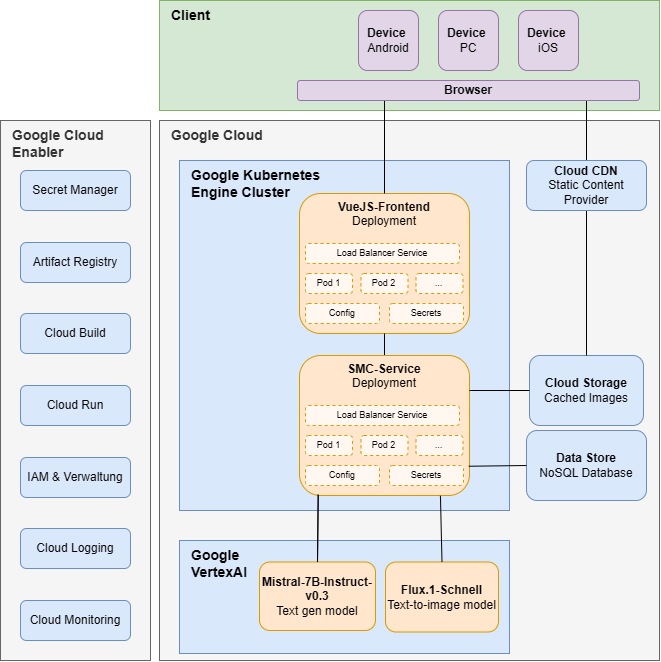
\includegraphics[width=0.8\textwidth]{abbildungen/Drawio/SystemArchitektur}
    \caption{Abbildung der Systemarchitektur}
    \label{fig:sytem-architektur}
    \raggedright Quelle: Eigene Darstellung
\end{figure}

\subsection{Antizipation der Kosten und des Nutzens}

Zur Berechnung der variablen Kosten im produktiven Betrieb der Plattform sind verschiedene Facetten zu betrachten, darunter die entstehenden Kosten für das Generieren und
speichern von Bild- und Textinhalten, die anfallenden Betriebskosten durch in Anspruchsnahme von Cloud Services sowie später anfallende Personalkosten für die Wartung und Weiterentwicklung der Plattform.

Um die Kostenstruktur der Plattform zu schätzen, werden verschiedene Szenarien betrachtet, welche die Kosten der Applikation unterschiedlich beeinflussen.
Dabei wird zwischen einem Best Case, einem Worst Case und einem realistischen Szenario unterschieden, welche sich maßgeblich durch die erwarten Nutzerzahlen unterscheiden.
Für die nachfolgende Kostenschätzung werden folgende Nutzerzahlen angenommen:

\begin{itemize}
    \item Best Case: 5000 User
    \item Worst Case: 50 User
    \item Realistisches Szenario: 500 User
\end{itemize}

\textbf{Generierung und Speicherung von Bildern}\newline
Zum Generieren der Bilder wird das Text-to-Image-Modell Flux-1-Schnell verwendet, welches auf der Google Cloud Plattform als Endpunkt bereitgestellt wird.
Dabei wird als Maschine ein in Belgien gehostetes n1-standard-4 gewählt, welches 4 \ac{vCPU} und 15 \ac{GB} \ac{RAM} besitzt.
Dies ist die kleinstmögliche Konfiguration für das Modell und verursacht Kosten von 0,24 \ac{USD} pro aufgewendete Maschinenstunde.\footcite{GoogleVertexAI2025}

Im Testbetrieb des Prototypen lag die Inferenzzeit pro Anfrage bei ca. 500 ms.
Basierend auf den festgelegten Szenarien ergibt sich folgende Kostenstruktur, bei der Annahme, dass jeder User 10 Anfragen pro Monat stellt:

\begin{itemize}
    \item Best Case: 5000 User * 10 Anfragen * 0,5 s * 0,24 \ac{USD} = 600 \ac{USD}
    \item Worst Case: 50 User * 10 Anfragen * 0,5 s * 0,24 \ac{USD} = 6 \ac{USD}
    \item Realistisches Szenario: 500 User * 10 Anfragen * 0,5 s * 0,24 \ac{USD} = 60 \ac{USD}
\end{itemize}

Die generierten Bilder werden im Google Cloud Storage gespeichert.
Dieser wird in der Region Belgien gehostet und wird mit 0,02 \ac{USD} pro \ac{GB} und Monat berechnet.\footcite{GoogleCloudStorage2025}

Die im Testbetrieb erzeugten Bilder hatten eine Größe von ca. 128 \ac{KB}.
Basierend auf den festgelegten Szenarien ergibt sich folgende Kostenstruktur:
\begin{itemize}
    \item Best Case: 5000 User * 10 Anfragen * 128 \ac{KB} * 0,02 \ac{USD} = 12,8 \ac{USD}
    \item Worst Case: 50 User * 10 Anfragen * 128 \ac{KB} * 0,02 \ac{USD} = 0,128 \ac{USD}
    \item Realistisches Szenario: 500 User * 10 Anfragen * 128 \ac{KB} * 0,02 \ac{USD} = 1,28 \ac{USD}
\end{itemize}

Der Speicherbedarf für generierte Bilder steigt neben dem eintretendem Szenario ebenso mit der Zeit an.
Dabei ist zu beachten, dass die Kosten für den Speicherplatz im Google Cloud Storage mit der Zeit steigen.

Auf die ersten drei Jahre sind dabei folgende Kosten zu erwarten:

\begin{figure}[htbp]
    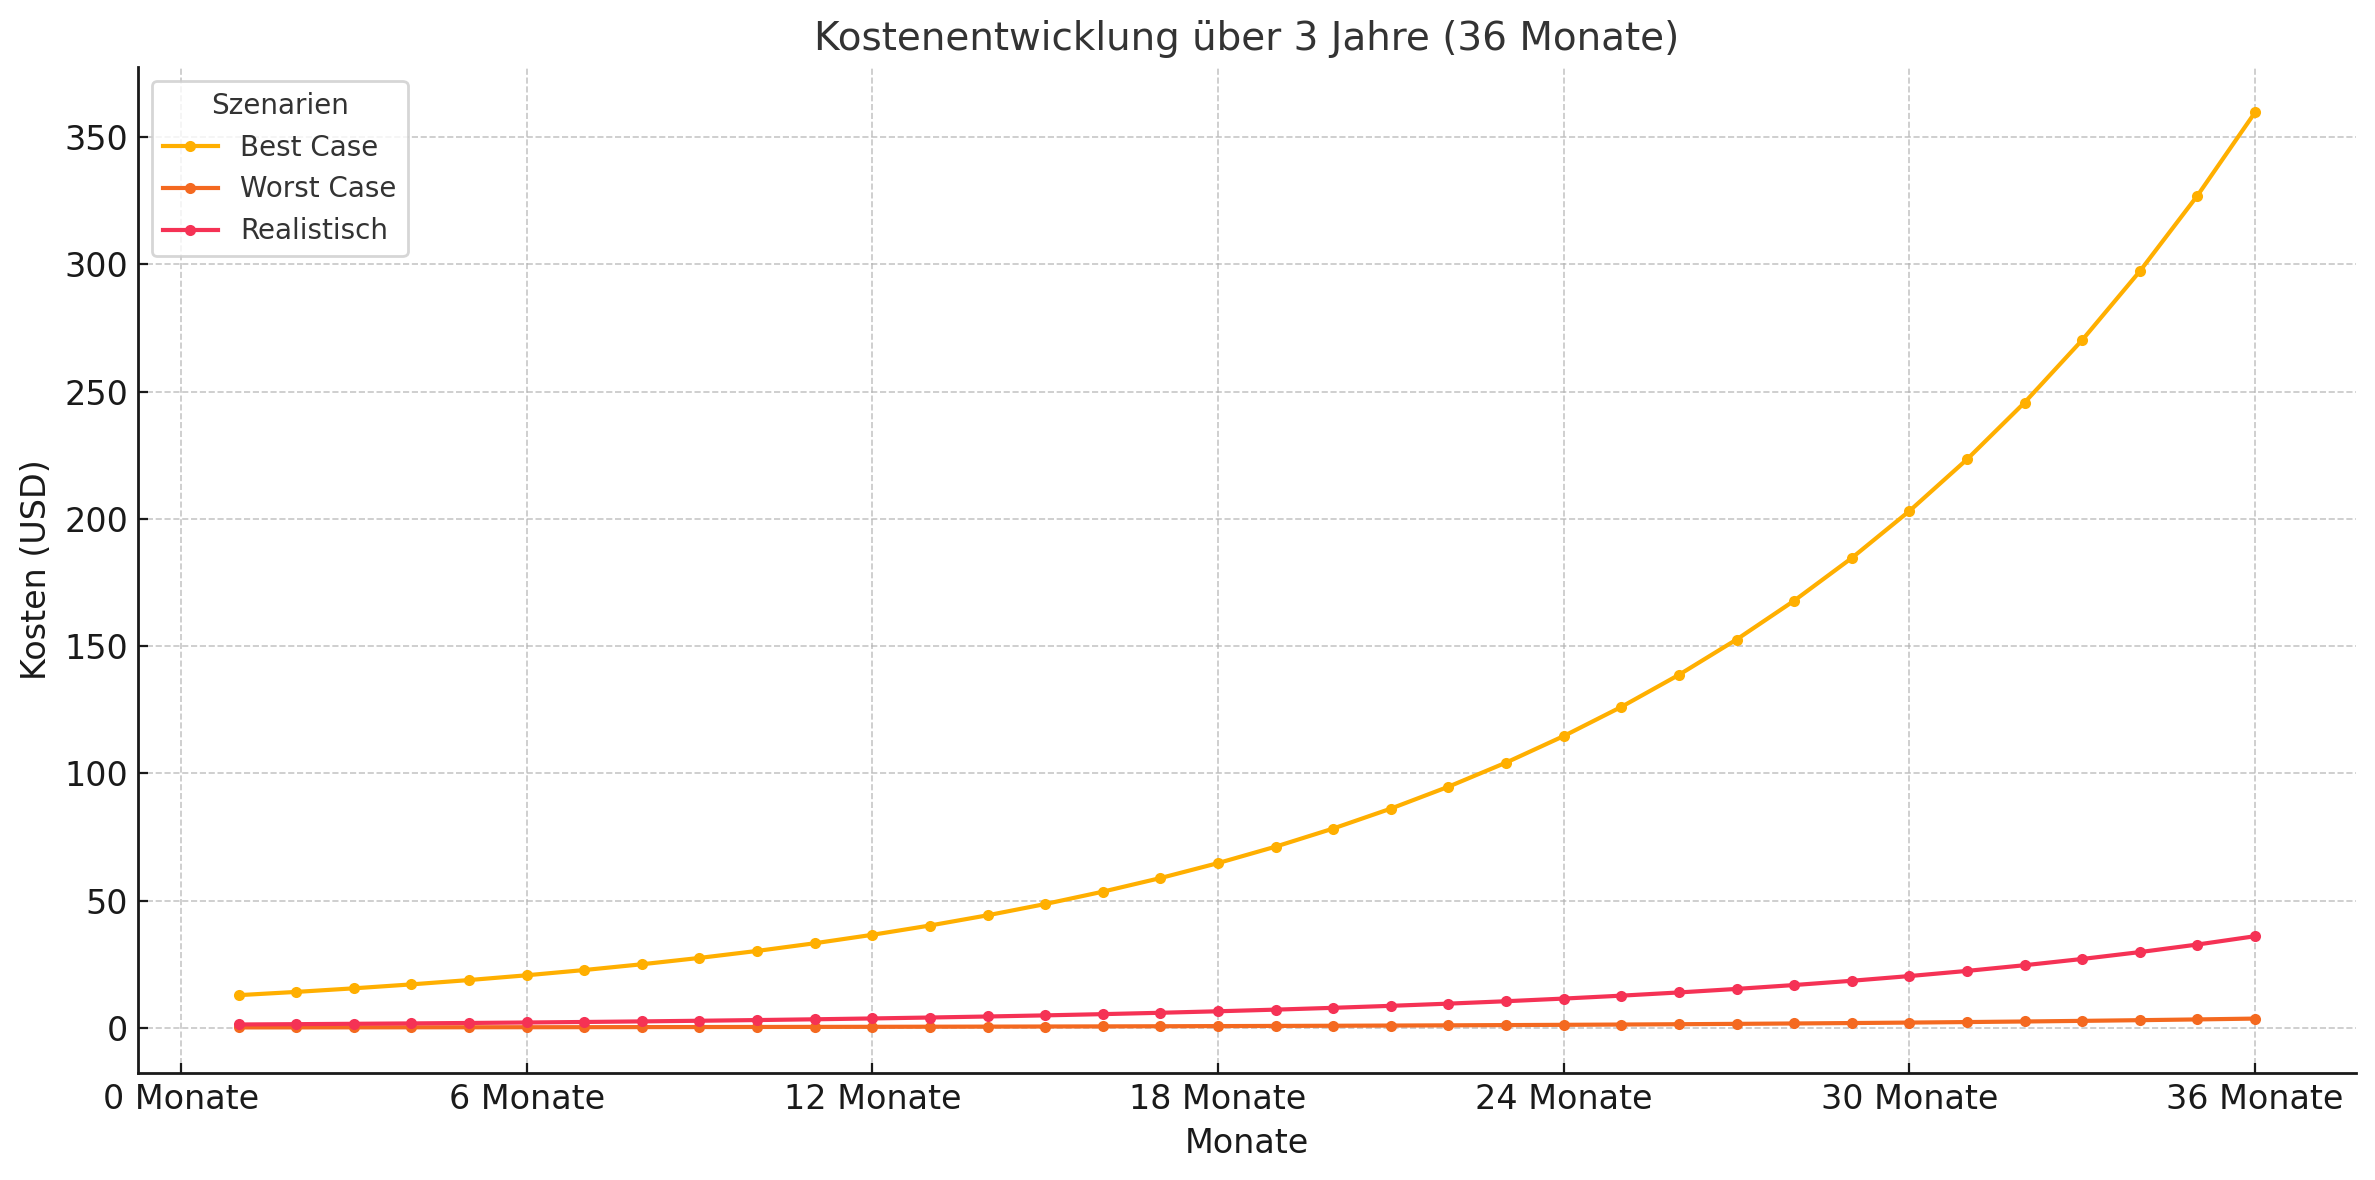
\includegraphics[width=\textwidth, height=\textheight, keepaspectratio]{abbildungen/KostenSpeicher}
    \caption{Kostenentwicklung für die Speicherung von Bildern über 3 Jahre}
    \label{fig:KostenentwicklungSpeicher}
    \raggedright Quelle: Eigene Darstellung
\end{figure}

\textbf{Generierung und Speicherung von Texten}\newline
Die Textgenerierung wird mit dem Text-to-Text-Modell Mistral-7B-Instruct durchgeführt, welches ebenfalls auf der Google Cloud Plattform als Endpunkt bereitgestellt wird.
Dabei wird die gleiche Konfiguration wie beim Bildmodell verwendet, entsprechend Region Belgien und n1-standard-4 als Maschine.
Die anfallenden Maschinenstunden werden jedoch geringer angenommen, da die Inferenzzeit pro Anfrage im Testbetrieb bei ca. 100 ms lag.

Daraus ergeben sich folgende Kostenstrukturen:
\begin{itemize}
    \item Best Case: 5000 User * 10 Anfragen * 0,1 s * 0,24 \ac{USD} = 120 \ac{USD}
    \item Worst Case: 50 User * 10 Anfragen * 0,1 s * 0,24 \ac{USD} = 1,2 \ac{USD}
    \item Realistisches Szenario: 500 User * 10 Anfragen * 0,1 s * 0,24 \ac{USD} = 12 \ac{USD}
\end{itemize}

Zum Speichern der generierten Texte wird der Data Store verwendet.
Dieser wird in der Region Belgien gehostet und wird nach Lese- und Schreibvorgängen, sowie den gespeicherten Daten berechnet.

\begin{figure}[htbp]
    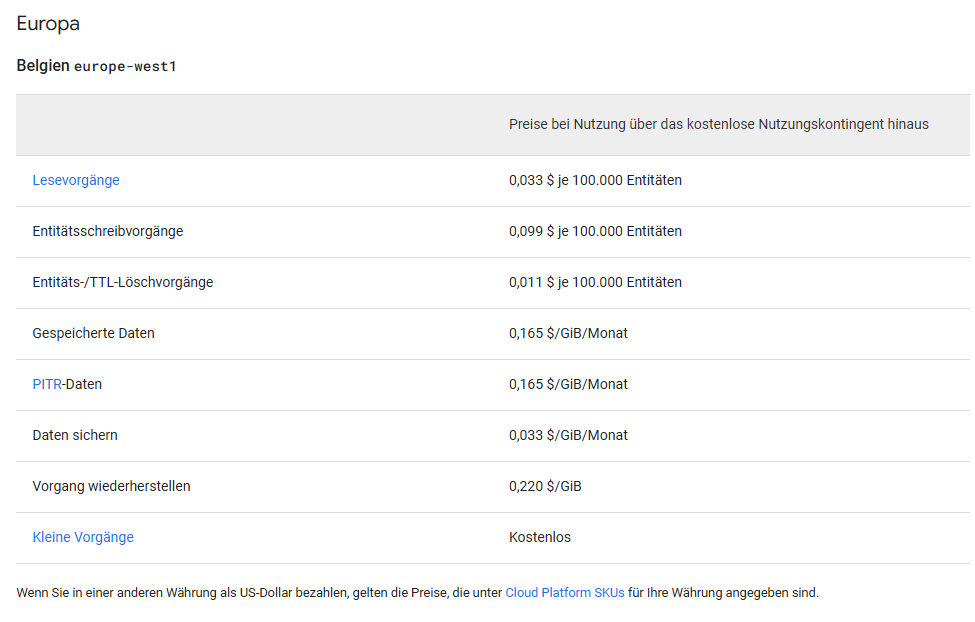
\includegraphics[width=\textwidth, height=\textheight, keepaspectratio]{abbildungen/kostendatastore}
    \caption{Kostenstruktur Data Store}
    \label{fig:KostenDataStore}
    \raggedright Quelle:\cite{GoogleDatastorePricing2025}
\end{figure}


Dabei wird nur die Nutzung abgerechnet, welche die Freikontingente überschreitet.
Dies wird einzig im Best Case Szenario eintreten, da die Freikontingente für die anderen Szenarien ausreichen.
Selbst im Best Case Szenario ist anzunehmen, dass einzig das Freikontingent für Schreibvorgänge minimal überschritten wird.
Dieses wird pro 100.000 Schreibvorgängen mit 0,099 \ac{USD} berechnet, weshalb diese Kosten vernachlässigbar sind.

Für den Speicherbedarf ist zu beachten, dass der Text bei einem Social Media Post bei durchschnittlich 200 Zeichen liegen kann.

\begin{itemize}
    \item \textbf{Best Case}
    \begin{itemize}
        \item \textbf{2025:} \(5000 \, \text{User} \times 24 \, \text{kB} = 117,19 \, \text{MB}\)
        \item \textbf{2026:} \(117,19 \, \text{MB} + (6000 \, \text{User} \times 24 \, \text{kB}) = 263,06 \, \text{MB}\)
        \item \textbf{2027:} \(263,06 \, \text{MB} + (7200 \, \text{User} \times 24 \, \text{kB}) = 440,25 \, \text{MB}\)
    \end{itemize}

    \item \textbf{Realistic Case}
    \begin{itemize}
        \item \textbf{2025:} \(500 \, \text{User} \times 24 \, \text{kB} = 11,72 \, \text{MB}\)
        \item \textbf{2026:} \(11,72 \, \text{MB} + (600 \, \text{User} \times 24 \, \text{kB}) = 26,31 \, \text{MB}\)
        \item \textbf{2027:} \(26,31 \, \text{MB} + (720 \, \text{User} \times 24 \, \text{kB}) = 44,03 \, \text{MB}\)
    \end{itemize}

    \item \textbf{Worst Case}
    \begin{itemize}
        \item \textbf{2025:} \(50 \, \text{User} \times 24 \, \text{kB} = 1,17 \, \text{MB}\)
        \item \textbf{2026:} \(1,17 \, \text{MB} + (60 \, \text{User} \times 24 \, \text{kB}) = 2,63 \, \text{MB}\)
        \item \textbf{2027:} \(2,63 \, \text{MB} + (72 \, \text{User} \times 24 \, \text{kB}) = 4,40 \, \text{MB}\)
    \end{itemize}
\end{itemize}

Daraus ergeben sich folgende Kosten in den kommenden drei Jahren:
\begin{figure}[htbp]
    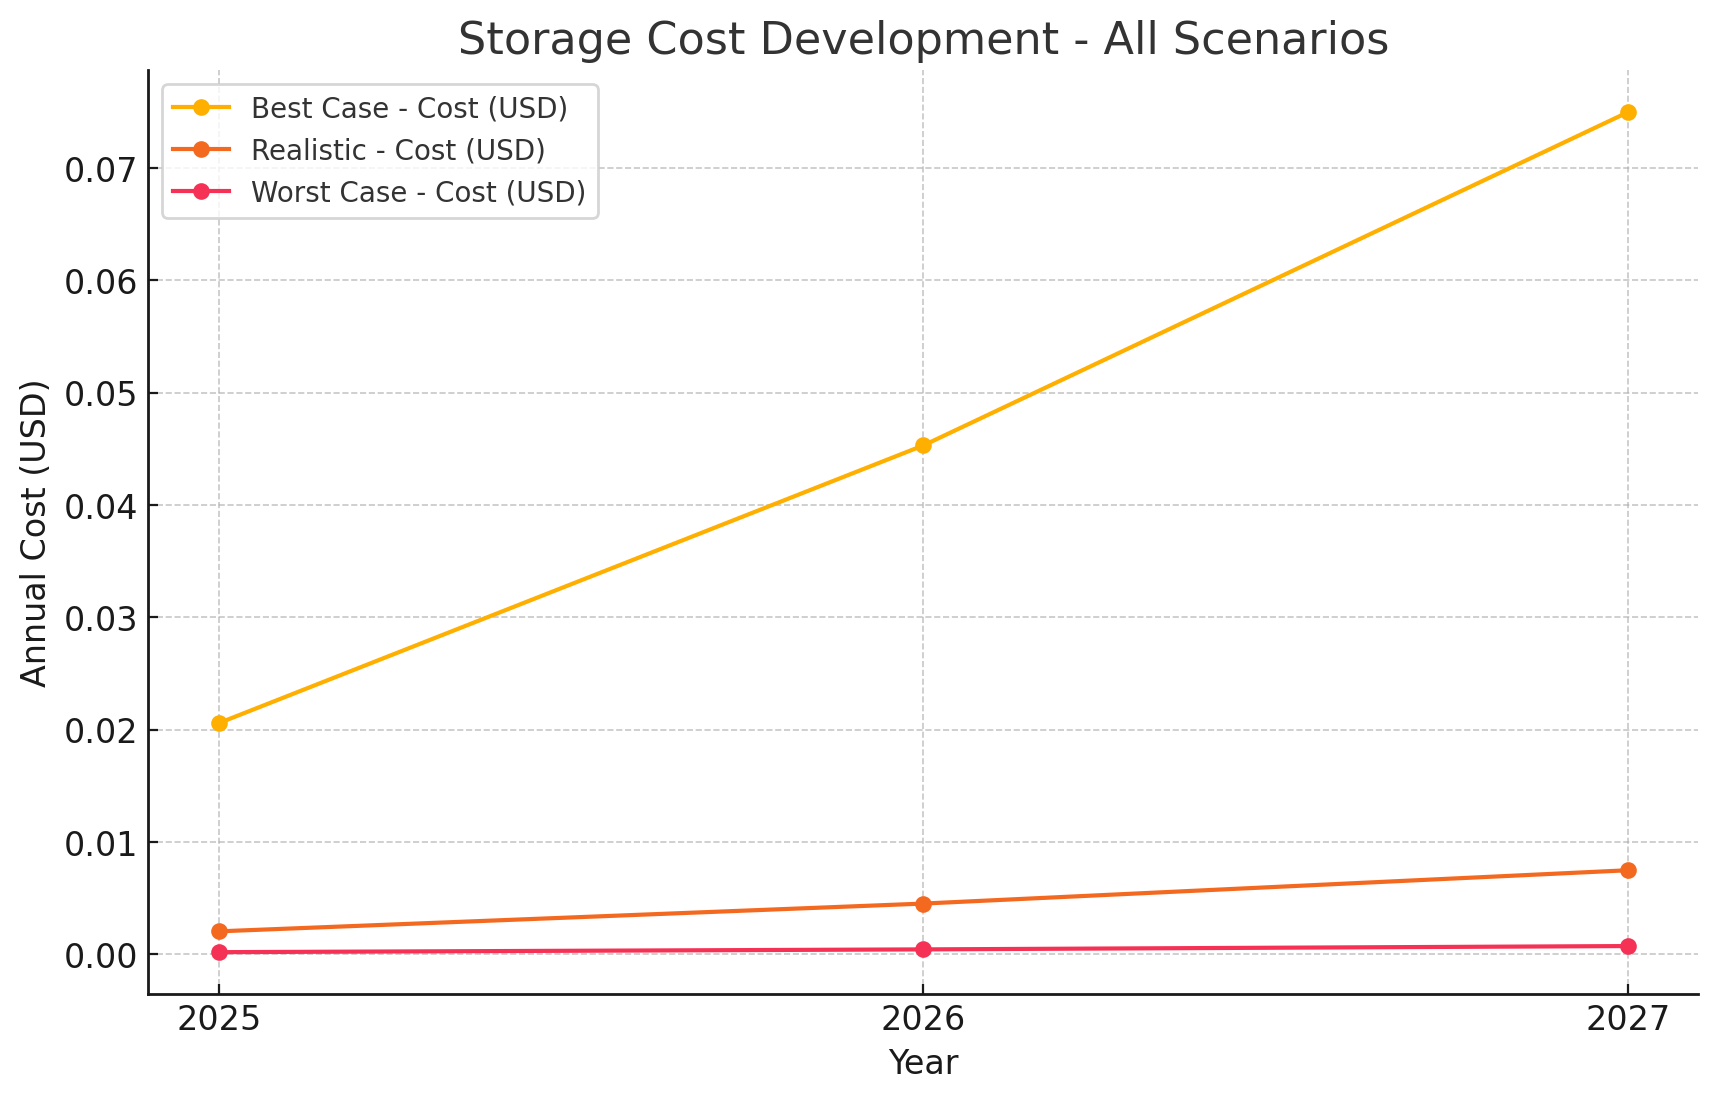
\includegraphics[width=\textwidth, height=\textheight, keepaspectratio]{abbildungen/Kosten_Speicher_Text}
    \caption{Entwicklung der Speicherkosten für Texte über 3 Jahre}
    \label{fig:KostenentwicklungSpeicherText}
    \raggedright Quelle: Eigene Darstellung
\end{figure}

Dabei ist über die Jahre bereits ein realisiertes Wachstum betrachtet, welches sich in den Kosten widerspiegelt.
Dennoch sind selbst im Best Case Szenario die Kosten für den Speicherplatz im Data Store vernachlässigbar.

\textbf{Plattform}\newline
Die Plattform setzt sich aus folgenden Komponenten zusammen:
\begin{itemize}
    \item Google Kubernetes Engine Cluster
    \item Google Cloud CDN
    \item Enabler Services (Monitoring, Logging, IAM, Secret Manager)
\end{itemize}

In der Ramp-Up-Phase wird die Plattform mit einer minimalen Konfiguration betrieben.
Die Funktion der Enterprise-Version sind für die ersten drei Jahre nicht notwendig und werden daher nicht betrachtet.
Dementsprechend wird die Standardversion von der Google Kubernetes Engine verwendet, welche 0,10 \ac{USD} pro Stunde kostet.\footcite{GoogleKubernetesEnginePricing2025}
Bei einem Betrieb von 24 Stunden am Tag ergeben sich folgende Kosten für die drei Jahre:

0,10 \ac{USD} * 24 h * 365 Tage * 3 Jahre = 2628 \ac{USD}

Zusätzlich sind die Kosten für die Enabler Services zu betrachten.

Für das Monitoring werden Kosten erhoben, basierend auf dem benötigen Speicher, sowie dem Aufrufen der erhobenen Daten.

\begin{itemize}
    \item 0,2580 \ac{USD}/MiB: erste 150–100.000 \ac{USD}/MiB
    \item 0,1510 \ac{USD}/MiB: nächste 100.000–250.000 \ac{USD}/MiB
    \item 0,0610 \ac{USD}/MiB: >250.000 \ac{USD}/MiB
\end{itemize}

Die Aufrufe werden mit 0,01 \ac{USD}/1.000API-Leseaufruf abgerechnet, wobei API-Schreibaufrufe kostenlos sind.

Die Plattform setzt sich aus drei Kubernetes Deployments zusammen.
Diese werden mit jeweils 2 Pods betrieben, um eine hohe Verfügbarkeit zu gewährleisten.
Daraus lässt sich ein grober Bedarf an Speicher von 1 GB ableiten, welcher für die ersten drei Jahre ausreicht.
Dieser lässt sich mit unterschiedlichen Speicherzeitrahmen reduzieren.
Wenn die Monitoring-Daten für 30 Tage gespeichert werden, ergibt sich ein Speicherbedarf von ca. 84,11 MiB.
Wird dieser auf die Kostenstruktur angewendet, ergeben sich näherungsweise folgende Kosten für die drei Jahre:

0,2580 \ac{USD}/MiB * 84,11 MiB * 365 Tage * 3 Jahre = 7,5 \ac{USD}

Zur Vereinfachung der Berechnung werden ähnliche Kosten für das Logging angenommen.

Für die Nutzung des \ac{IAM} Services fallen keine Kosten an.\footcite{GoogleIAMPricing2025}
Für den Secret Manager ist in der Standardversion eine Nutzung von 100 Secrets kostenlos, weshalb auch hier keine Kosten anfallen.\footcite{GoogleSecretManagerPricing2025}

\textbf{Personalkosten}\newline
Für die Weiterentwicklung des Produktes werden zwei Entwickler benötigt.
Für den Betrieb des Produktes, im Sinne von Support, wird ein Service-Desk Mitarbeiter benötigt.
Die Kosten für einen Entwickler belaufen sich auf 100€ die Stunde und für einen Service-Desk Mitarbeiter auf 35€ die Stunde.


\textbf{Entwicklungskosten}\newline
Zur Entwicklung der Plattform sind nach Abschluss dieser Arbeit noch folgende Arbeiten notwendig, um ein produktiven Betrieb zu gewährleisten:
\begin{itemize}
    \item Entwicklung und Anpassung der Frontend-Applikation
    \item Anpassen der Kubernetes Deployments
    \item Einrichten der Enabler Services
    \item Einrichten des Data Store + Google Cloud Storage
    \item Einrichten des \ac{CDN}
    \item Ende-zu-Ende-Tests
    \item Aufbau Support- und Wartungsstruktur
\end{itemize}

Zur Berechnung der Entwicklungskosten sind folgende Annahmen zu treffen:
\begin{itemize}
    \item Stundensatz Entwickler: 100 Euro
    \item Entwicklungsteam: 5 Entwickler
\end{itemize}

Zur Erfassung der Aufwände werden grobe \ac{FTE} angenommen, welche die Entwicklungskosten für die ersten drei Jahre darstellen.
Damit ergeben sich folgende Kosten:
\begin{itemize}
    \item Entwicklung und Anpassung der Frontend-Applikation - 5 \ac{FTE}
    \item Anpassen der Kubernetes Deployments - 2 \ac{FTE}
    \item Einrichten der Enabler Services - 2 \ac{FTE}
    \item Einrichten des Data Store + Google Cloud Storage - 1 \ac{FTE}
    \item Einrichten des CDN - 1 \ac{FTE}
    \item Ende-zu-Ende-Tests - 5 \ac{FTE}
    \item Aufbau Support- und Wartungsstruktur 3 \ac{FTE}
\end{itemize}

Daraus ergeben sich grob folgende Personalkosten:
19 \ac{FTE} * 8 Stunden * 100 Euro = 15.200 Euro

Zusätzlich sind die Kosten für die Entwicklungsumgebung zu betrachten.
Diese teilt sich in das Bereitstellen des notwendigen Toolings, sowie einer Testumgebung auf.
Da die restaufwände lediglich ein kleines Team bestehend aus 5 Entwicklern benötigen, fallen keine nennenswerten Kosten für die Entwicklungsumgebung an.
Einzig relevant sind die Lizenzkosten für die benötigten Entwicklungsumgebungen, welche mit 100 Euro pro Entwickler pro Monat angenommen werden.

Um die finalen Aufwände leisten zu können wird ein Zeitraum von 2 Monaten angenommen, in welchem die Entwicklung abgeschlossen wird.
Daraus ergeben sich folgende Kosten:
5 Entwickler * 100 Euro * 2 Monate = 1000 Euro

Zusammenfassend ergeben sich folgende Entwicklungskosten:
15.200 Euro + 1000 Euro = 16.200 Euro

%(Pricing Modell Auswahl)

Das Freemium-Bezahlmodell, bei welchem Nutzer der Applikation erst nach einer gewissen Anzahl von Social-Media-Posts monatlich bezahlen müssen, bietet eine Möglichkeit die Kosten für den Betrieb und die Entwicklung der Anwendung zu amortisieren.
Die Kosten für die Premiumvariante sind so zu wählen, dass sie die Betriebskosten tragen können und eine Gewinnmarge erwirtschaftet werden kann.
Gleichzeitig muss bei der Preisgestaltung berücksichtigt werden, dass man diese nicht zu hoch ansetzt und diese in Relation zu den Wettbewerbern steht.
Kilian, die Applikation, welche auf Contentgenerierung innerhalb der Gastronomie- und Hotelbranche spezialisiert ist, nimmt mit der Premiumvariante mindestens 23€ pro Monat ein.
Die Lösung des Unternehmens MARA nimmt für seine GenAI-basierende Lösung in der Premiumvariante je Zugang 99€ pro Monat ein.
Jasper stellt sich mit zwei verschieden Varianten auf, der Startervariante mit 30€ pro Monat und der Boss-Mode-Variante mit 60€ pro Monat.
Unter der Betrachtung der Konkurrenten wird ein Einstandspreis von 20€ pro Monat bestimmt, damit diese Lösung die günstigste am Markt ist und viele Kunden anlocken kann.
Unter der Betrachtung der drei skizzierten Szenarien (50, 500, 5000 Nutzer) könnten folgende Ertragskalkulationen eintreffen:

50 Nutzer + 20€ pro Monat = 1.000€ pro Monat
500 Nutzer + 20€ pro Monat = 10.000€ pro Monat
5000 Nutzer +20€ pro Monat = 100.000€ pro Monat

%(Sonstige Einnahmen)

Ein weiterer Aspekt in der Einnahme spiegeln die erhobenen Daten, wie die Prompts und generierten Social-Media-Posts, wider.
Diese können ein Einblick in die Gastronomie vermitteln und wichtige Rückschlüsse für die Entwicklung von Produkten suggerieren.
Dementsprechend könnten diese Daten von hohem Interesse für Unternehmen sein, die ggf. selber in die Gastronomie einsteigen wollen oder Produkte für die Gastronomie entwickeln wollen.
Der Wert dieser Daten bestimmt sich im Volumen und Qualität der abgegebenen Daten.
Da sich die Applikation in den Anfängen befindet, wird der Verkauf von Nutzerdaten erstmal nicht betrachtet.

%(Break Even Analyse)
Eine Break-Even-Analyse erlaubt die Betrachtung, ab welchem Zeitpunkt sich der Betrieb der Lösung wirtschaftlich rentiert.
Die Betrachtung erfolgt auf monatlicher Basis.
Das impliziert, dass sämtliche Kosten auf einen monatlichen Faktor runtergebrochen werden, ebenso, wie die Erträge.
Daraus ergibt sich, dass die Anwendung ca. 3760 zahlende Nutzer benötigt, um den Break-Even-Point zu erreichen.

\begin{figure}[htbp]
    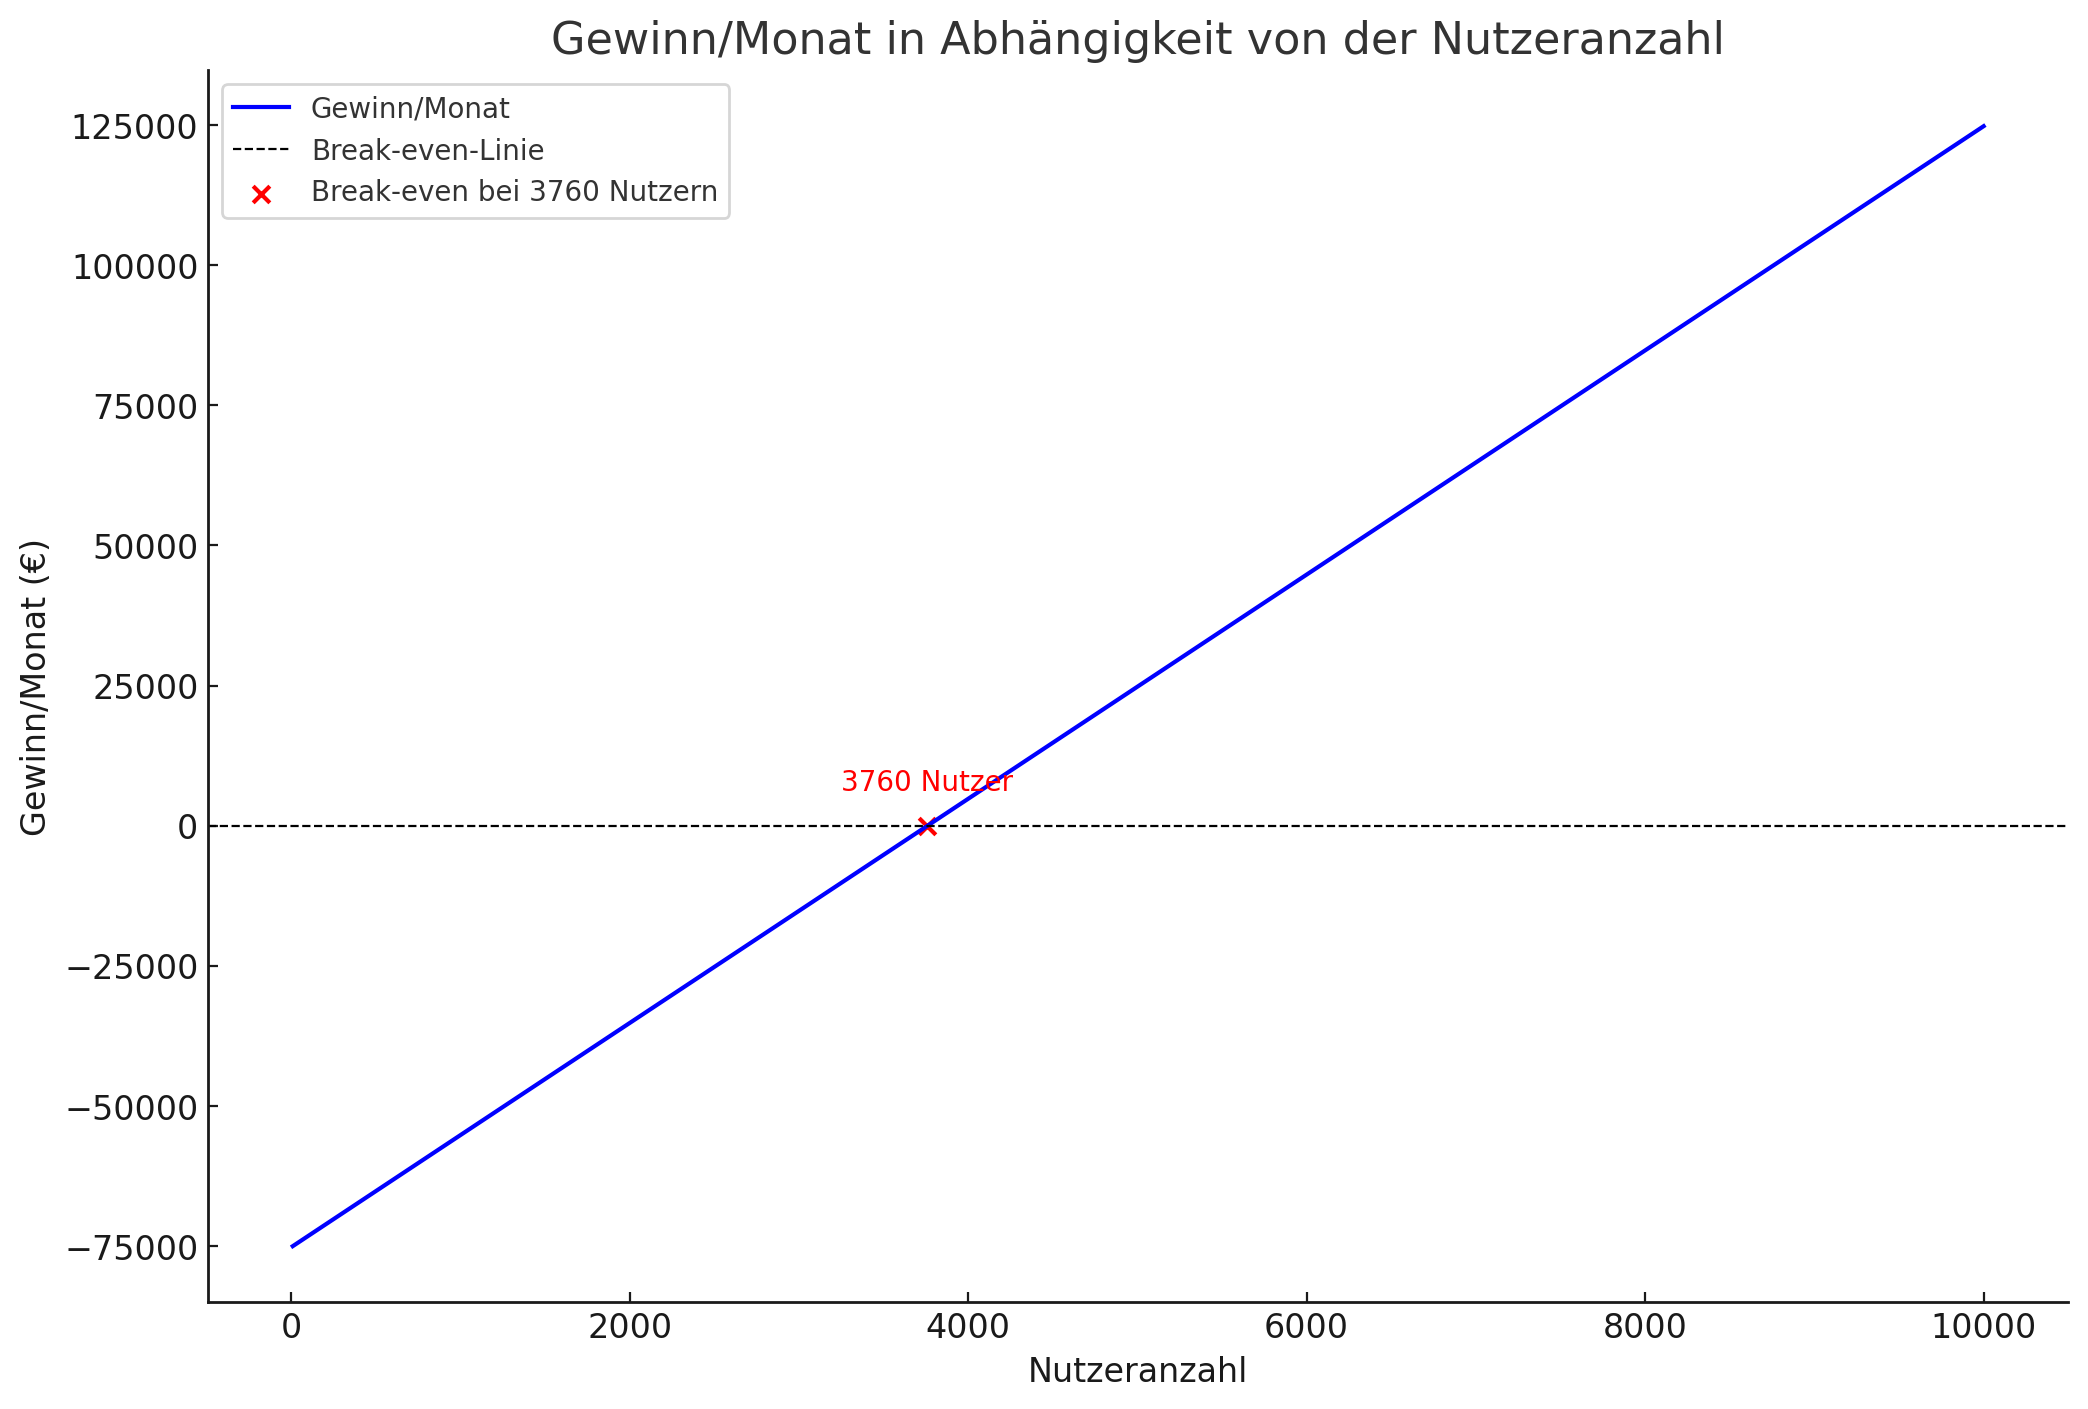
\includegraphics[width=\textwidth, height=\textheight, keepaspectratio]{abbildungen/Break_Even}
    \caption{Break Even Analyse}
    \label{fig:BreakEven}
    \raggedright Quelle: Eigene Darstellung
\end{figure}